\begin{figure}[H]
    \centering


    \tikzset{every picture/.style={line width=0.75pt}} %set default line width to 0.75pt

    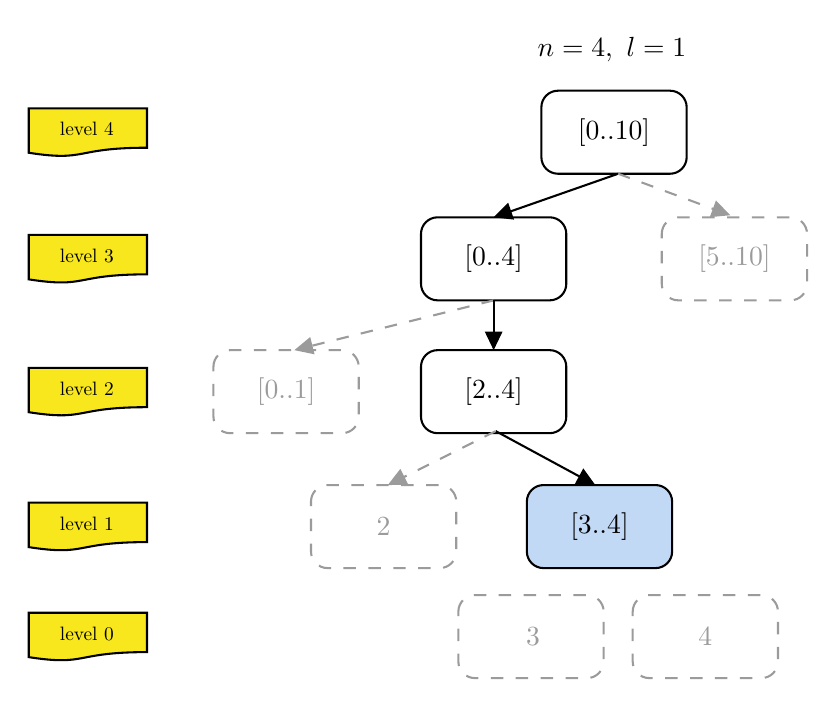
\begin{tikzpicture}[x=0.75pt,y=0.75pt,yscale=-1,xscale=1]
        %uncomment if require: \path (0,340); %set diagram left start at 0, and has height of 340

        %Rounded Rect [id:dp41297758491075554]
        \draw  [color={rgb, 255:red, 0; green, 0; blue, 0 }  ,draw opacity=1 ] (284,48) .. controls (284,43.58) and (287.58,40) .. (292,40) -- (346,40) .. controls (350.42,40) and (354,43.58) .. (354,48) -- (354,72) .. controls (354,76.42) and (350.42,80) .. (346,80) -- (292,80) .. controls (287.58,80) and (284,76.42) .. (284,72) -- cycle ;
        %Rounded Rect [id:dp6520424082590635]
        \draw   (226,109) .. controls (226,104.58) and (229.58,101) .. (234,101) -- (288,101) .. controls (292.42,101) and (296,104.58) .. (296,109) -- (296,133) .. controls (296,137.42) and (292.42,141) .. (288,141) -- (234,141) .. controls (229.58,141) and (226,137.42) .. (226,133) -- cycle ;
        %Rounded Rect [id:dp17376535076708577]
        \draw  [color={rgb, 255:red, 155; green, 155; blue, 155 }  ,draw opacity=1 ][dash pattern={on 4.5pt off 4.5pt}] (342,109) .. controls (342,104.58) and (345.58,101) .. (350,101) -- (404,101) .. controls (408.42,101) and (412,104.58) .. (412,109) -- (412,133) .. controls (412,137.42) and (408.42,141) .. (404,141) -- (350,141) .. controls (345.58,141) and (342,137.42) .. (342,133) -- cycle ;
        %Rounded Rect [id:dp6626394915573943]
        \draw   (226,173) .. controls (226,168.58) and (229.58,165) .. (234,165) -- (288,165) .. controls (292.42,165) and (296,168.58) .. (296,173) -- (296,197) .. controls (296,201.42) and (292.42,205) .. (288,205) -- (234,205) .. controls (229.58,205) and (226,201.42) .. (226,197) -- cycle ;
        %Rounded Rect [id:dp6613554759465123]
        \draw  [color={rgb, 255:red, 155; green, 155; blue, 155 }  ,draw opacity=1 ][dash pattern={on 4.5pt off 4.5pt}] (126,173) .. controls (126,168.58) and (129.58,165) .. (134,165) -- (188,165) .. controls (192.42,165) and (196,168.58) .. (196,173) -- (196,197) .. controls (196,201.42) and (192.42,205) .. (188,205) -- (134,205) .. controls (129.58,205) and (126,201.42) .. (126,197) -- cycle ;
        %Rounded Rect [id:dp18103482508891444]
        \draw  [color={rgb, 255:red, 155; green, 155; blue, 155 }  ,draw opacity=1 ][dash pattern={on 4.5pt off 4.5pt}] (173,238) .. controls (173,233.58) and (176.58,230) .. (181,230) -- (235,230) .. controls (239.42,230) and (243,233.58) .. (243,238) -- (243,262) .. controls (243,266.42) and (239.42,270) .. (235,270) -- (181,270) .. controls (176.58,270) and (173,266.42) .. (173,262) -- cycle ;
        %Rounded Rect [id:dp6156099131399975]
        \draw  [color={rgb, 255:red, 0; green, 0; blue, 0 }  ,draw opacity=1 ][fill={rgb, 255:red, 193; green, 217; blue, 245 }  ,fill opacity=1 ] (277,238) .. controls (277,233.58) and (280.58,230) .. (285,230) -- (339,230) .. controls (343.42,230) and (347,233.58) .. (347,238) -- (347,262) .. controls (347,266.42) and (343.42,270) .. (339,270) -- (285,270) .. controls (280.58,270) and (277,266.42) .. (277,262) -- cycle ;
        %Straight Lines [id:da940569460881393]
        \draw    (321,80) -- (262.89,100.34) ;
        \draw [shift={(261,101)}, rotate = 340.71000000000004] [fill={rgb, 255:red, 0; green, 0; blue, 0 }  ][line width=0.75]  [draw opacity=0] (8.93,-4.29) -- (0,0) -- (8.93,4.29) -- cycle    ;

        %Straight Lines [id:da19886917638438795]
        \draw [color={rgb, 255:red, 155; green, 155; blue, 155 }  ,draw opacity=1 ] [dash pattern={on 4.5pt off 4.5pt}]  (321,80) -- (373.12,99.31) ;
        \draw [shift={(375,100)}, rotate = 200.32] [fill={rgb, 255:red, 155; green, 155; blue, 155 }  ,fill opacity=1 ][line width=0.75]  [draw opacity=0] (8.93,-4.29) -- (0,0) -- (8.93,4.29) -- cycle    ;

        %Straight Lines [id:da7809582170361684]
        \draw [color={rgb, 255:red, 155; green, 155; blue, 155 }  ,draw opacity=1 ] [dash pattern={on 4.5pt off 4.5pt}]  (261,141) -- (166.94,164.51) ;
        \draw [shift={(165,165)}, rotate = 345.96000000000004] [fill={rgb, 255:red, 155; green, 155; blue, 155 }  ,fill opacity=1 ][line width=0.75]  [draw opacity=0] (8.93,-4.29) -- (0,0) -- (8.93,4.29) -- cycle    ;

        %Straight Lines [id:da49593042124322273]
        \draw    (261,141) -- (261,163) ;
        \draw [shift={(261,165)}, rotate = 270] [fill={rgb, 255:red, 0; green, 0; blue, 0 }  ][line width=0.75]  [draw opacity=0] (8.93,-4.29) -- (0,0) -- (8.93,4.29) -- cycle    ;

        %Straight Lines [id:da07216174009388476]
        \draw    (262,204) -- (308.24,229.05) ;
        \draw [shift={(310,230)}, rotate = 208.44] [fill={rgb, 255:red, 0; green, 0; blue, 0 }  ][line width=0.75]  [draw opacity=0] (8.93,-4.29) -- (0,0) -- (8.93,4.29) -- cycle    ;

        %Straight Lines [id:da9300341613494139]
        \draw [color={rgb, 255:red, 155; green, 155; blue, 155 }  ,draw opacity=1 ] [dash pattern={on 4.5pt off 4.5pt}]  (262,204) -- (211.79,229.11) ;
        \draw [shift={(210,230)}, rotate = 333.43] [fill={rgb, 255:red, 155; green, 155; blue, 155 }  ,fill opacity=1 ][line width=0.75]  [draw opacity=0] (8.93,-4.29) -- (0,0) -- (8.93,4.29) -- cycle    ;

        %Flowchart: Document [id:dp6500761765411522]
        \draw  [fill={rgb, 255:red, 248; green, 231; blue, 28 }  ,fill opacity=1 ] (37,48.5) -- (94,48.5) -- (94,67.47) .. controls (58.38,67.47) and (65.5,74.32) .. (37,69.89) -- cycle ;

        %Flowchart: Document [id:dp5580407874202131]
        \draw  [fill={rgb, 255:red, 248; green, 231; blue, 28 }  ,fill opacity=1 ] (37,109.5) -- (94,109.5) -- (94,128.48) .. controls (58.38,128.48) and (65.5,135.32) .. (37,130.89) -- cycle ;

        %Flowchart: Document [id:dp3741114720480607]
        \draw  [fill={rgb, 255:red, 248; green, 231; blue, 28 }  ,fill opacity=1 ] (37,173.5) -- (94,173.5) -- (94,192.48) .. controls (58.38,192.48) and (65.5,199.32) .. (37,194.89) -- cycle ;

        %Flowchart: Document [id:dp020109097297930534]
        \draw  [fill={rgb, 255:red, 248; green, 231; blue, 28 }  ,fill opacity=1 ] (37,238.5) -- (94,238.5) -- (94,257.48) .. controls (58.38,257.48) and (65.5,264.32) .. (37,259.89) -- cycle ;

        %Flowchart: Document [id:dp06728244444869125]
        \draw  [fill={rgb, 255:red, 248; green, 231; blue, 28 }  ,fill opacity=1 ] (37,291.5) -- (94,291.5) -- (94,310.48) .. controls (58.38,310.48) and (65.5,317.32) .. (37,312.89) -- cycle ;

        %Rounded Rect [id:dp005401328342101053]
        \draw  [color={rgb, 255:red, 155; green, 155; blue, 155 }  ,draw opacity=1 ][dash pattern={on 4.5pt off 4.5pt}] (244,291) .. controls (244,286.58) and (247.58,283) .. (252,283) -- (306,283) .. controls (310.42,283) and (314,286.58) .. (314,291) -- (314,315) .. controls (314,319.42) and (310.42,323) .. (306,323) -- (252,323) .. controls (247.58,323) and (244,319.42) .. (244,315) -- cycle ;
        %Rounded Rect [id:dp20978566864575288]
        \draw  [color={rgb, 255:red, 155; green, 155; blue, 155 }  ,draw opacity=1 ][dash pattern={on 4.5pt off 4.5pt}] (328,291) .. controls (328,286.58) and (331.58,283) .. (336,283) -- (390,283) .. controls (394.42,283) and (398,286.58) .. (398,291) -- (398,315) .. controls (398,319.42) and (394.42,323) .. (390,323) -- (336,323) .. controls (331.58,323) and (328,319.42) .. (328,315) -- cycle ;

        % Text Node
        \draw (318,20) node  [align=left] {$\displaystyle n=4,\ l=1$};
        % Text Node
        \draw (377,121) node [color={rgb, 255:red, 155; green, 155; blue, 155 }  ,opacity=1 ] [align=left] {[5..10]};
        % Text Node
        \draw (261,121) node  [align=left] {[0..4]};
        % Text Node
        \draw (319,60) node [color={rgb, 255:red, 0; green, 0; blue, 0 }  ,opacity=1 ] [align=left] {[0..10]};
        % Text Node
        \draw (261,185) node  [align=left] {[2..4]};
        % Text Node
        \draw (161,185) node [color={rgb, 255:red, 155; green, 155; blue, 155 }  ,opacity=1 ] [align=left] {[0..1]};
        % Text Node
        \draw (208,250) node [color={rgb, 255:red, 155; green, 155; blue, 155 }  ,opacity=1 ] [align=left] {2};
        % Text Node
        \draw (312,250) node  [align=left] {[3..4]};
        % Text Node
        \draw (65,58.5) node [scale=0.7] [align=left] {level 4};
        % Text Node
        \draw (65,119.5) node [scale=0.7] [align=left] {level 3};
        % Text Node
        \draw (65,183.5) node [scale=0.7] [align=left] {level 2};
        % Text Node
        \draw (65,248.5) node [scale=0.7] [align=left] {level 1};
        % Text Node
        \draw (65,301.5) node [scale=0.7] [align=left] {level 0};
        % Text Node
        \draw (280,303) node [color={rgb, 255:red, 155; green, 155; blue, 155 }  ,opacity=1 ] [align=left] {3};
        % Text Node
        \draw (363,303) node [color={rgb, 255:red, 155; green, 155; blue, 155 }  ,opacity=1 ] [align=left] {4};


    \end{tikzpicture}
    \caption{Range generalizer example}\label{fig:range_generalizer}
\end{figure}